\documentclass[12pt,a4paper]{article}
\usepackage[utf8]{inputenc}
\usepackage[margin=1in]{geometry}
\usepackage{amsmath}
\usepackage{amsfonts}
\usepackage{amssymb}
\usepackage{graphicx}
\usepackage{listings}
\usepackage{xcolor}
\usepackage{fancyhdr}
\usepackage{titlesec}
\usepackage{enumitem}
\usepackage{tikz}
\usepackage{circuitikz}

% Arduino syntax highlighting
\lstdefinelanguage{Arduino}{
  language=C++,
  morekeywords={String, digitalWrite, delay, pinMode, analogRead, digitalRead, Serial, HIGH, LOW, INPUT, OUTPUT},
  sensitive=true,
  morecomment=[l]//,
  morecomment=[s]{/*}{*/},
  morestring=[b]",
}

\lstdefinestyle{arduinostyle}{
    language=Arduino,
    basicstyle=\ttfamily\small,
    keywordstyle=\color{blue}\bfseries,
    commentstyle=\color{green!50!black},
    stringstyle=\color{red},
    numbers=left,
    numberstyle=\tiny\color{gray},
    numbersep=5pt,
    breaklines=true,
    breakatwhitespace=true,
    tabsize=2,
    showspaces=false,
    showstringspaces=false,
    frame=single,
    rulecolor=\color{gray!30},
    backgroundcolor=\color{gray!5}
}

\lstset{style=arduinostyle}

\pagestyle{fancy}
\fancyhf{}
\rhead{ESP32 IoT Project}
\lhead{Visitor Counter}
\cfoot{\thepage}

\titleformat{\section}{\Large\bfseries}{\thesection}{1em}{}
\titleformat{\subsection}{\large\bfseries}{\thesubsection}{1em}{}

\begin{document}

\begin{center}
    \LARGE \textbf{Bidirectional Visitor Counter using ESP32, IR Sensors, Buzzer, LED and Blynk App}
    
    \large Project Report and Documentation
\end{center}

\vspace{1cm}

\section{Circuit Diagram}

\begin{center}
    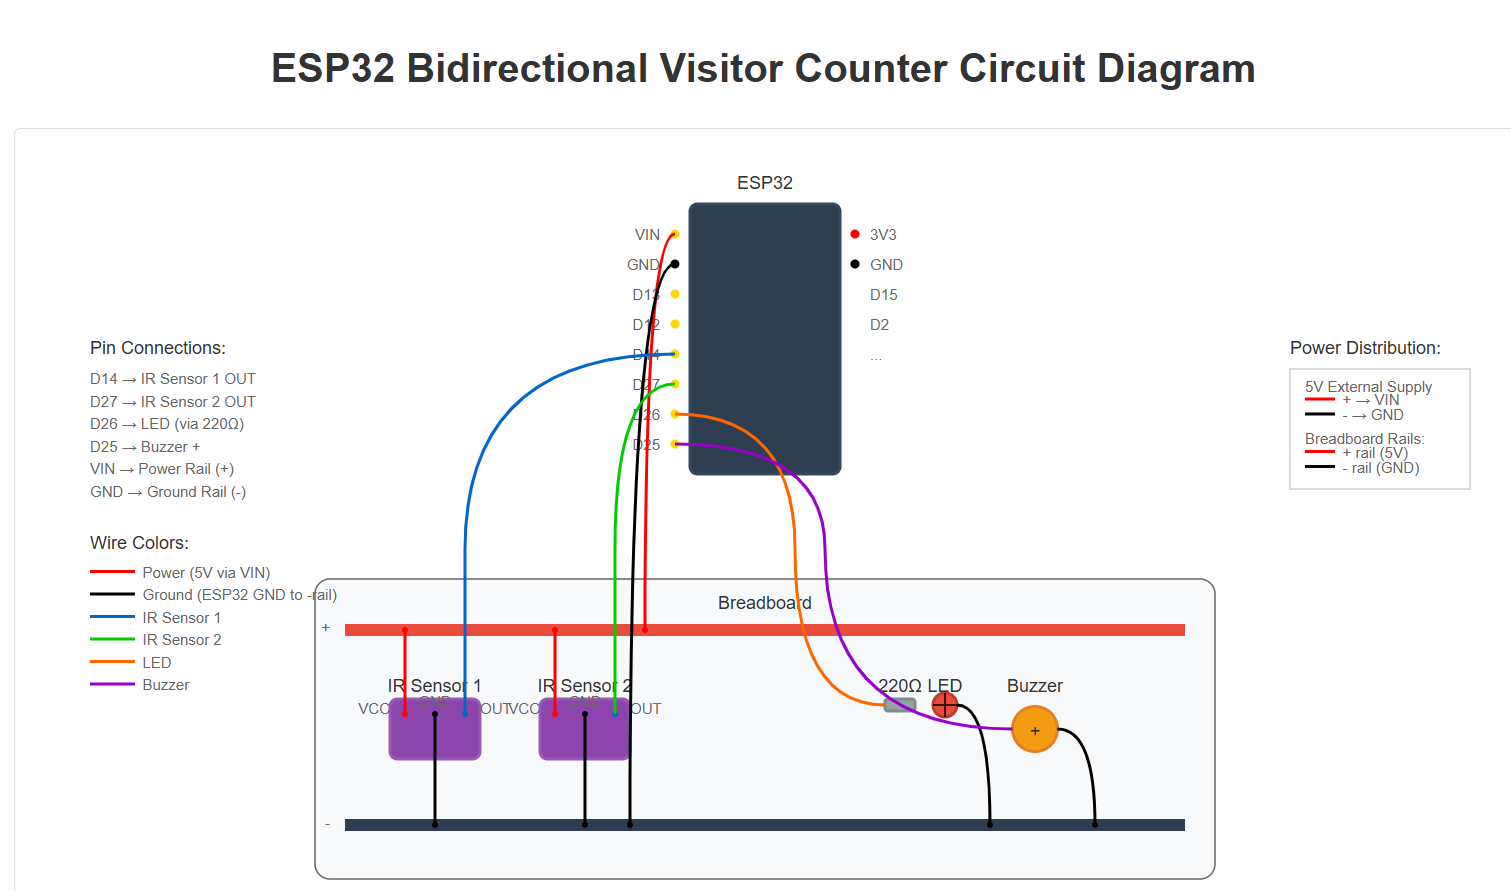
\includegraphics[width=1\textwidth]{diagram.png}
\end{center}


\subsection{Component List}
\begin{itemize}[leftmargin=*]
    \item ESP32 Development Board
    \item 2× IR Obstacle Avoidance Sensors
    \item 1× LED (any color)
    \item 1× 220Ω Resistor
    \item 1× Active Buzzer (3-5V)
    \item 1× Breadboard
    \item Jumper wires (Male-to-Male and Male-to-Female)
\end{itemize}
\newpage

\subsection{Pin Connection Summary}
\\
\begin{table}[h!]
\centering
\begin{tabular}{|l|l|l|}
\hline
\textbf{Component} & \textbf{Pin} & \textbf{ESP32 Pin} \\
\hline
IR Sensor 1 & OUT & D14 \\
IR Sensor 2 & OUT & D27 \\
LED & Anode (+) & D26 (via 220Ω resistor) \\
Buzzer & Positive (+) & D25 \\
All Components & VCC/+ & 3.3V \\
All Components & GND/- & GND \\
\hline
\end{tabular}
\caption{Pin Connection Table}
\end{table}

\section{Arduino Code}
\begin{lstlisting}
#define BLYNK_PRINT Serial

#define BLYNK_TEMPLATE_ID "TMPL6fTt5tuUg"
#define BLYNK_TEMPLATE_NAME "Bidirectional Visitor Counter"
#define BLYNK_AUTH_TOKEN "VXuRa-O8gETyth0bwScmeDtL0NASoAwZ"

#include <WiFi.h>
#include <BlynkSimpleEsp32.h>

// Blynk Auth Token
char auth[] = "VXuRa-O8gETyth0bwScmeDtL0NASoAwZ";
// WiFi credentials - Use your home's WiFi name and password here
char ssid[] = "kingFisher";
char pass[] = "BortY8728@";

// Pin Configuration
#define IR_SENSOR_1 14
#define IR_SENSOR_2 27
#define LED_PIN     26
#define BUZZER_PIN  25

// Variables
int count = 0;
const int threshold = 10; //for sound buzzer
bool lastIR1 = HIGH, lastIR2 = HIGH;
unsigned long lastTriggerTime = 0;
const unsigned long debounceDelay = 300; // ms

void setup() {
  Serial.begin(115200);
  pinMode(IR_SENSOR_1, INPUT_PULLUP);
  pinMode(IR_SENSOR_2, INPUT_PULLUP);
  pinMode(LED_PIN, OUTPUT);
  pinMode(BUZZER_PIN, OUTPUT);
  digitalWrite(LED_PIN, LOW);
  digitalWrite(BUZZER_PIN, LOW);

  Blynk.begin(auth, ssid, pass);
}

void loop() {
  Blynk.run();

  bool ir1 = digitalRead(IR_SENSOR_1) == HIGH;
  bool ir2 = digitalRead(IR_SENSOR_2) == HIGH;

  enum State { IDLE, IR1_TRIGGERED, IR2_TRIGGERED } ;
  static State state = IDLE;
  static unsigned long firstTriggerTime = 0;
  const unsigned long sequenceTimeout = 10000;

  unsigned long now = millis();

  switch (state) {
    case IDLE:
      // Start entry sequence if IR1 triggers
      if (ir1 && !ir2) {
        state = IR1_TRIGGERED;
        firstTriggerTime = now;
      }
      // Start exit sequence if IR2 triggers
      else if (ir2 && !ir1) {
        state = IR2_TRIGGERED;
        firstTriggerTime = now;
      }
      break;

    case IR1_TRIGGERED:
      // Wait for IR2 to be triggered within the timeout for entry
      if (ir2 && now - firstTriggerTime < sequenceTimeout) {
        count++;
        Serial.println("Entry detected");
        updateDevices();
        state = IDLE;
      }
      // If sensors released or timeout passed, reset
      else if ((!ir1 && !ir2) || (now - firstTriggerTime >= sequenceTimeout)) {
        state = IDLE;
      }
      break;

    case IR2_TRIGGERED:
      // Wait for IR1 to be triggered within the timeout for exit
      if (ir1 && now - firstTriggerTime < sequenceTimeout) {
        if (count > 0) count--;
        Serial.println("Exit detected");
        updateDevices();
        state = IDLE;
      }
      // If sensors released or timeout passed, reset
      else if ((!ir1 && !ir2) || (now - firstTriggerTime >= sequenceTimeout)) {
        state = IDLE;
      }
      break;
  }
}


void updateDevices() {
  // Light control
  digitalWrite(LED_PIN, count > 0 ? HIGH : LOW);
  // Buzzer control
  if (count >= threshold) {
    digitalWrite(BUZZER_PIN, HIGH);
    delay(500);
    digitalWrite(BUZZER_PIN, LOW);
  }
  // Blynk updates
  Blynk.virtualWrite(V0, count); // Value Display widget
  Blynk.virtualWrite(V1, count > 0 ? 255 : 0); // LED widget
}

BLYNK_WRITE(V2) {
  if (param.asInt() == 1) {
    count = 0;
    updateDevices();
    Serial.println("Count reset via Blynk image button");
  }
}
\end{lstlisting}

\section{Code Explanation}

\begin{itemize}[leftmargin=*]
  \item \textbf{Blynk and WiFi Setup:} Auth token, WiFi SSID, and password are initialized.
  \item \textbf{Pin Definitions:} IR sensors on D14 and D27, LED on D26, and buzzer on D25.
  \item \textbf{Visitor Logic:} Uses a finite state machine (FSM) to detect entry and exit sequences based on IR sensor trigger order.
  \item \textbf{updateDevices():} Updates LED, buzzer, and sends virtual pin values to Blynk app.
  \item \textbf{BLYNK\_WRITE():} Resets count if virtual pin V2 is pressed from Blynk image button.
\end{itemize}

\section{Hardware Connections (ESP32 + Breadboard)}

\subsection*{ESP32 Pin Layout}
\begin{itemize}
  \item \textbf{EN side (connected to breadboard):} VIN, GND, D13, D12, D14, D27, D26, D25
  \item \textbf{BOOT side (open):} 3V3, GND, D15, D2, etc.
\end{itemize}

\subsection*{Wiring Instructions}

\begin{enumerate}
  \item \textbf{Power}
  \begin{itemize}
    \item 3.3V (BOOT side) → Breadboard positive rail (male-to-female wire)
    \item GND (BOOT side) → Breadboard negative rail (male-to-female wire)
  \end{itemize}

  \item \textbf{IR Sensor 1 (connected to D14)}
  \begin{itemize}
    \item VCC → Breadboard + rail
    \item GND → Breadboard - rail
    \item OUT → D14 (male-to-male)
  \end{itemize}

  \item \textbf{IR Sensor 2 (connected to D27)}
  \begin{itemize}
    \item VCC → Breadboard + rail
    \item GND → Breadboard - rail
    \item OUT → D27 (male-to-male)
  \end{itemize}

  \item \textbf{LED (connected to D26)}
  \begin{itemize}
    \item Anode (+, longer leg) → Resistor → D26 (male-to-male)
    \item Cathode (-, shorter leg) → GND rail
  \end{itemize}

  \item \textbf{Buzzer (connected to D25)}
  \begin{itemize}
    \item + → D25 (male-to-male)
    \item - → GND rail
  \end{itemize}
\end{enumerate}

\subsection*{Jumper Wire Types}
\begin{itemize}
  \item Male-to-Male: Breadboard to ESP32 inserted pins
  \item Male-to-Female: ESP32 BOOT side pins to breadboard power rails
\end{itemize}

\section{Project Features}

\subsection{Bidirectional Detection}
The system uses two IR sensors positioned in sequence to detect the direction of movement:
\begin{itemize}
  \item \textbf{Entry:} IR Sensor 1 triggered first, then IR Sensor 2
  \item \textbf{Exit:} IR Sensor 2 triggered first, then IR Sensor 1
\end{itemize}

\subsection{Visual and Audio Feedback}
\begin{itemize}
  \item \textbf{LED Indicator:} Turns ON when count > 0, OFF when count = 0
  \item \textbf{Buzzer Alert:} Activates when visitor count reaches threshold (10 people)
\end{itemize}

\subsection{IoT Integration}
\begin{itemize}
  \item \textbf{Blynk App:} Real-time monitoring via smartphone
  \item \textbf{Virtual Pins:} V0 (count display), V1 (LED status), V2 (reset button)
  \item \textbf{Remote Reset:} Count can be reset remotely via Blynk app
\end{itemize}

\section{Blynk App Configuration}

\subsection{Virtual Pin Setup}
\begin{table}[h!]
\centering
\begin{tabular}{|c|l|l|}
\hline
\textbf{Virtual Pin} & \textbf{Widget} & \textbf{Function} \\
\hline
V0 & Value Display & Shows current visitor count \\
V1 & LED Widget & Visual indicator (ON/OFF) \\
V2 & Button Widget & Reset counter to zero \\
\hline
\end{tabular}
\caption{Blynk Virtual Pin Configuration}
\end{table}

\subsection{Required Blynk Credentials}
\begin{itemize}
  \item Template ID: TMPL6fTt5tuUg
  \item Template Name: Bidirectional Visitor Counter
  \item Auth Token: VXuRa-O8gETyth0bwScmeDtL0NASoAwZ
\end{itemize}

\section{How It Works}

\subsection{Finite State Machine Logic}
The system operates using a three-state finite state machine:

\begin{enumerate}
  \item \textbf{IDLE State:} Waiting for sensor trigger
  \item \textbf{IR1\_TRIGGERED:} First sensor activated, waiting for second
  \item \textbf{IR2\_TRIGGERED:} Second sensor activated, waiting for first
\end{enumerate}

\subsection{Detection Sequence}
\begin{itemize}
  \item When a person approaches from outside:
    \begin{enumerate}
      \item IR Sensor 1 detects person → State changes to IR1\_TRIGGERED
      \item IR Sensor 2 detects person → Count increments → State returns to IDLE
    \end{enumerate}
  \item When a person exits from inside:
    \begin{enumerate}
      \item IR Sensor 2 detects person → State changes to IR2\_TRIGGERED  
      \item IR Sensor 1 detects person → Count decrements → State returns to IDLE
    \end{enumerate}
\end{itemize}

\subsection{Timeout Protection}
A 10-second timeout prevents false counts from incomplete sequences or sensor noise.

\section{Troubleshooting}

\subsection{Common Issues}
\begin{itemize}
  \item \textbf{Sensors not responding:} Check 3.3V power supply and ground connections
  \item \textbf{False counts:} Adjust sensor sensitivity potentiometers or increase timeout
  \item \textbf{Blynk connection issues:} Verify WiFi credentials and auth token
  \item \textbf{LED/Buzzer not working:} Check pin connections and component polarity
\end{itemize}

\subsection{Calibration Tips}
\begin{itemize}
  \item Position sensors 50-80cm apart for optimal detection
  \item Adjust sensor height to waist level (80-100cm from ground)
  \item Test detection range by adjusting onboard potentiometers
  \item Ensure sensors face each other across the doorway
\end{itemize}

\section{Future Enhancements}

\begin{itemize}
  \item Data logging with timestamps
  \item Email/SMS notifications when threshold is reached
  \item Web dashboard for historical data analysis
  \item Battery backup for power outages
  \item Multiple room monitoring with additional sensor pairs
\end{itemize}


The system provides an affordable and scalable solution for visitor monitoring in various applications including retail stores, offices, exhibitions, and smart home automation.

\end{document}